Synthify is a music player that allows a user to bring all of their content from from different platforms \& services (YouTube, Spotify, SoundCloud, etc.) into one place

\subsection{Purpose and Use}
Synthify will allow users to sign in with different providers to fetch their content from the respective platforms. This will allow them to have all their content in one place. Synthify required users to provide their login information for each service that they want to connect to. If a user does not have an account with one of the music services that can be connected with Synthify and he/she wants to start using that service, he/she has to meet the requirement of that service.

\subsection{Intended Audience}
Synthify is open to anyone who wants to use the service. There is no hard Terms of Service for using the platform. However, the associated services that users will be signed in with to get their content have their own Terms of Service. We align our product with those respective Terms of Service and should a consumer choose to our product, they must also follow those terms.

\begin{figure}[h!]
	\centering
   	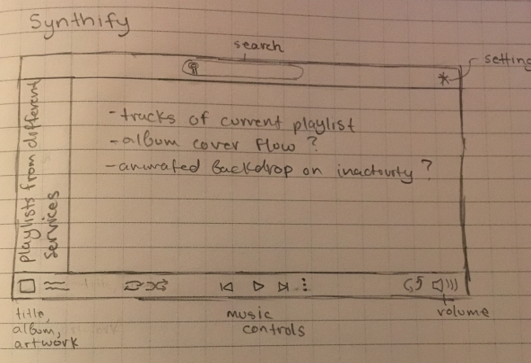
\includegraphics[width=0.60\textwidth]{images/concept.png}
    \caption{conceptual drawing}
\end{figure}
